%
% This file is part of PYCTS, the PY151 Credit Tracking System.
%
% PYCTS is free software: you can redistribute it and/or modify
% it under the terms of the GNU General Public License as published by
% the Free Software Foundation, either version 3 of the License, or
% (at your option) any later version.
%
% PYCTS is distributed in the hope that it will be useful,
% but WITHOUT ANY WARRANTY; without even the implied warranty of
% MERCHANTABILITY or FITNESS FOR A PARTICULAR PURPOSE.  See the
% GNU General Public License for more details.
%
% You should have received a copy of the GNU General Public License
% along with PYCTS.  If not, see <http://www.gnu.org/licenses/>.
%
% PYCTS and this file are Copyright 2011 by Mark Platek.
%

\documentclass[letterpaper]{article}

\usepackage[margin=2cm]{geometry}
\usepackage{graphicx}
\usepackage[small,compact]{titlesec}

% cause sections not to be numbered
\setcounter{secnumdepth}{-1} 

% set no paragraph indent and skip space between paragraphs
\setlength\parindent{0pt}
\setlength{\parskip}{8pt}

% no page numbers
\pagestyle{empty}

% PYCTS version
\newcommand{\softwareversion}{0.4.0.0}


\begin{document}

\begin{center}
{\bf {\huge PYCTS Primer for Students } }

Software Version: \softwareversion

Prepared for: Department of Psychology, Clarkson University
\end{center}

\section{What is PYCTS?}
PYCTS is web software that allows you to quickly and easily check the number of research credits you have earned. You can also use PYCTS to check what research studies are currently being offered to students.

\section{Where is PYCTS?}
PYCTS can be found at the following URL:

{\tt http://clarkson.edu/projects/researchcredit}

\section{How do I check my credits?}
Open a browser and go to the URL above, then log in using your Clarkson username and password. This is the same username and password you use to access other Clarkson web resources (such as Moodle and Peoplesoft). You will see a table of credits - each entry corresponds to one study you have participated in. In the following example, the student has a total of 3 credits, from participating in two studies.

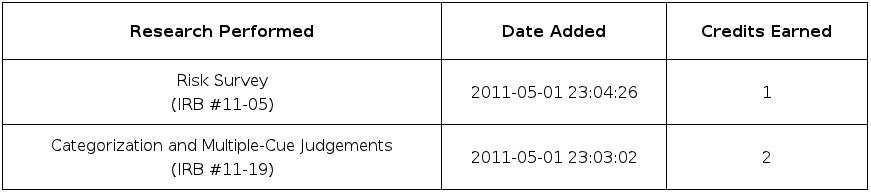
\includegraphics[width=\textwidth]{../images/student_main-screen.png}

\section{How can I find out what studies are available?}
If you want to participate in a study for credit, check the "Credit Opportunities" section after you have logged into PYCTS. You'll see a table of all credit-bearing research studies currently being offered to students. For each study, you can download a flyer containing more information (including a contact e-mail address or phone number). In the following example, several studies are available.

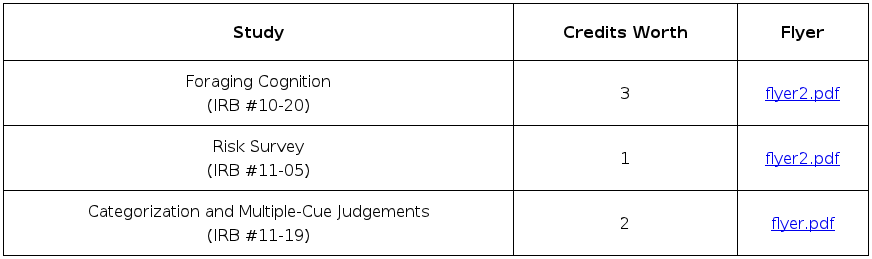
\includegraphics[width=\textwidth]{../images/student_studies.png}








\end{document}
